\documentclass[jou,apacite]{IEEEtran}
\usepackage{amsfonts}
\usepackage{amsthm}
\usepackage{tabu}
\usepackage{amssymb}
\usepackage{mathtools}
\usepackage{relsize}

\usepackage{minted}
\setminted{fontsize=\small} % numbers=right, bgcolor=lightgray}

\usepackage{graphicx}
\graphicspath{ {../images/} }
\setlength\parindent{0pt}

\title{Scala - A Powerful and Scalable Function-Objective Programming Language}

\author{Troy Hu and Benjamin Killeen} % alphabetical by last name

\begin{document}
\maketitle    
\begin{abstract}
Insert abstract here.
\end{abstract}                     

\section{Introduction}
\label{sec:intro}

During the mid 2000s, progress in developing component software was slow, which the researchers believed to be because existing languages had little support for component abstraction and composition. Some examples include statically typed languages such as Java and C\#. In response to this lack of progress, Odersky et al. designed and implemented Scala in order to develop better language support for component software. As the researchers put it, components ``are simply software parts which are used in some way by larger parts or whole applications. Components can take many forms; they can be modules, classes, libraries, frameworks, processes, or web services." At the same time, they envisioned their language as eventually being widely adopted. 


The researchers achieved their goals by focusing on two areas: 
\begin{itemize}
\item Developing scalable mechanisms for abstraction, composition, and
  decomposition. Through this focus, they made their language more scalable
  than existing languages such as Java. I.e., small and large components of
  component software can be expressed with the same concepts.
\item Combining functional programming and object-oriented
  programming. Odersky et al. decided to combine these two programming
  paradigms in order to prove better scalable support for software
  components.
\end{itemize}
We now describe on a high-level how Scala achieves its goals of providing
good support for component software and encouraging mass adoption.

\subsection{High-Level Design}
\label{sec:high-level-design}

In order to encourage adoption by software developers, Scala's syntax is very similar to Java's and C\#'s. In fact, Scala is able to work and interact with components coded in Java and C\#. However, remember that Java and C\# are suboptimal languages for supporting component software. Thus, in order to improve component support over Java and C\#, Scala discards or modifies some their existing conventions. For example, Figure 1 demonstrates a simple program (CITE THIS) that prints out options provided in the command line.
\begin{figure}[h]
  \centering
  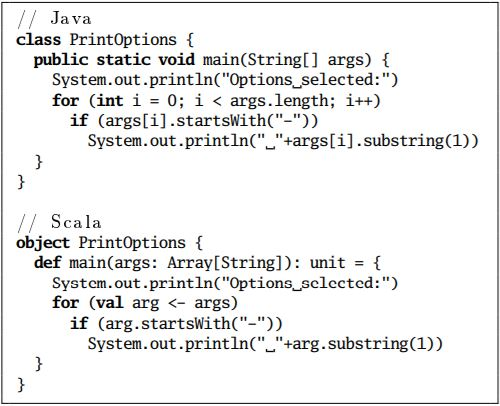
\includegraphics[width=\columnwidth]{print_options.JPG}
  \caption{Figure 1. Notice how Scala's general syntax and structure are similar
    to Java's. At the same time, there are some visible differences, e.g., unit
    is returned in the Scala implementation instead of void in the Java
    implementation. (CITE THIS IMAGE FROM OVERVIEW PAPER.)}
  \label{fig:example}
\end{figure}

Large parts of Scala's typing system are unique to the language. Scala's abstract type definitions and path-dependent types utilize $\nu$Obj Calculus (See Section III). Additionally, Scala implements modular mixin composition which combines the advantages of mixins and traits. Traits in Scala are essentially the equivalent of abstract classes in Java while mixins are classes/traits in which other non-child traits can draw methods from. \\\\
Scala also has a uniform object model. That is, every value is an object and
every operation is a call to a method. For example, the boolean “true” itself is
an object (S singleton object, in fact. See Section II for definition of
singleton object). At the same time, Scala includes functional programming
aspects such functions being first-class values (i.e. functions can be passed as
values) and pattern matching. For pattern matching specifically, Scala allows
objects themselves to be decomposed. This language also implements powerful and
novel abstraction concepts for types and values. For example, unlike Java
abstract classes, traits can include method implementations or fields.

% 3. related work
\section{Related Work}
\label{sec:related-work}

We did not know what $\nu$Obj calculus was and therefore read the paper “A
Nominal Theory of Objects with Dependent Types” by Martin Odersky, Vincent
Cremet, Christine Rockl, and Matthias Zenger to better understand the
concept. Because our main focus is specifically on understanding Scala and not
on learning the $\nu$Obj calculus (which itself is a topic worthy of its own
summary paper), we only provide a general description of $\nu$Obj calculus
below.
  
According to Odersky et al., $\nu$Obj calculus, broadly, is “a calculus and
dependent type system for classes and objects can have types as members.” Note
that a dependent type is a type that is defined by some value. The calculus’s
type system is well typed and can implement crucial aspects of Java’s inner
class system, virtual types, and family polymorphism. Moreover, this type system
can also model SML-style modules and functors. $\nu$Obj calculus diverges from
standard type systems for objects in three significant ways:

\begin{itemize}
\item Instead of only objects being primitive, classes are also primitive. We
  can view classes as “first class” as they can be the result of a term
  evaluation and be associated with labels.
\item Object records are not passed around during evaluation and type
  checking. Rather, every object has a name reference that is passed around.
\item Object types can be expressed using (possibly nominal) type components.
\end{itemize}
  
We leave Figures 2 (syntax) and 3 (type assignment) below for the reader's
interest.
\begin{figure}[h]
  \centering
  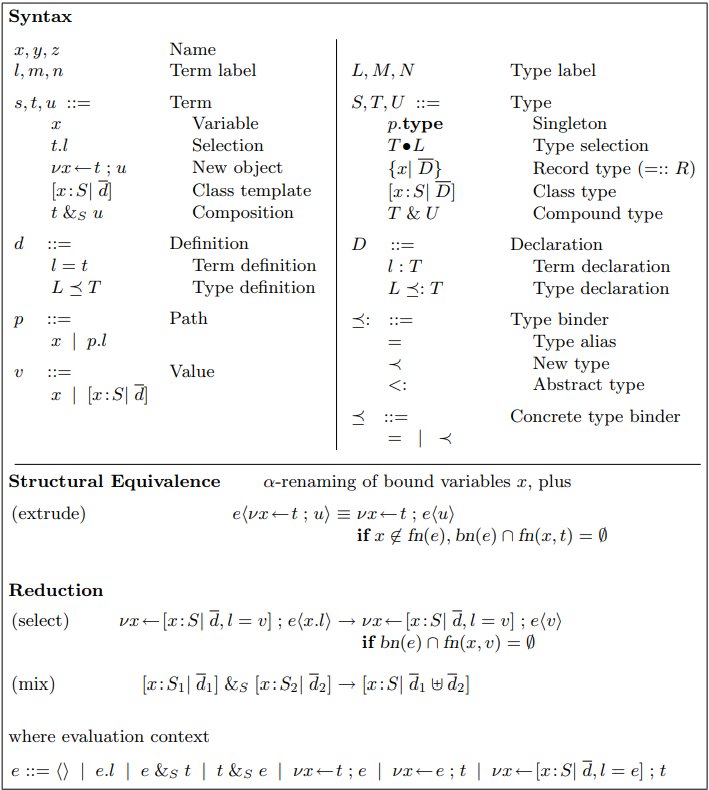
\includegraphics[width=\columnwidth]{syntax}
  \caption{The syntax of the $\nu$Obj calculus}
  \label{fig:example}
\end{figure}

\begin{figure}[h]
  \centering
  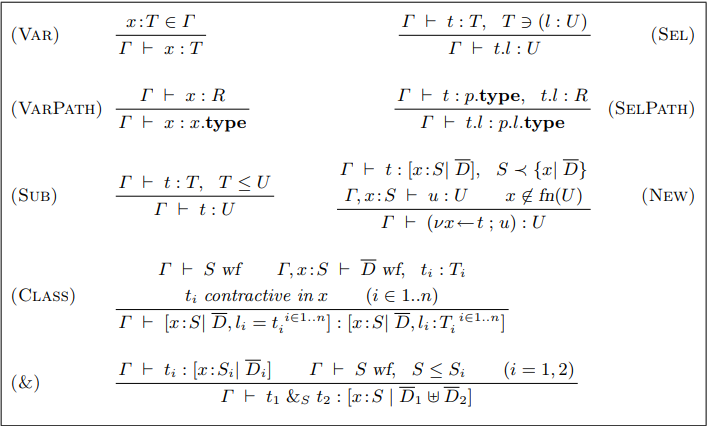
\includegraphics[width=\columnwidth]{typecheck}
  \caption{The typing rules of the $\nu$Obj calculus}
  \label{fig:example}
\end{figure}


% 2. Technical summary: Killeen
\section{Interesting Technical Details}
\label{sec:interesting-tech}

\begin{figure}
  
  \inputminted{Scala}{examples/nats.scala}
  \caption{An example outlining Scala classes.}
  \label{lst:nats-example}
\end{figure}

\subsection{Singleton Objects}
Scala is very unique in that it implements Singleton Objects. Singleton Objects are classes that can only have one instance while a Scala program is running. Such classes are defined almost exactly the same as normal Scala classes. The only difference is that the \texttt{class} modifier is replaced by the \texttt{object} modifier. Some examples of singleton objects include: a class representation of Zero and the PrintOptions example from above. Note that Singleton Objects are used extensively when Scala uses a Java class. Every static member of a Java class is stored in a Singleton Object.

\subsection{Unified Object Model}
In Scala, every value is an object and every class is a subtype of the \texttt{Any} class. Below the \texttt{Any} class, Scala classes can generally be divided into two groups: value classes that inherit from the \texttt{AnyVal} class and reference classes that inherit from the \texttt{AnyRef} class. Note that the value classes that are not \texttt{AnyVal} do not subtype each other. This means, for example, that the \texttt{Int} class is not a subtype of the \texttt{Float} class. Scala prevents such subtyping because the language forces an invariant that when a value is interpreted in a subclass and a super class, the values's representation does not change. For example, both \texttt{Int} and \texttt{Float} maintain a \texttt{MaxValue} member. However, the \texttt{MaxValue} of \texttt{Float} is different from the \texttt{MaxValue} of \texttt{Int}. Instead, Scala implements \textbf{views} (discussed below) which allow from implicit conversions from one type to another. As expected of an object-oriented language, class \texttt{Null} is a subtype of every reference type. However, since Scala is part functional, the language also has a \texttt{Nothing} type, which represents an empty type, is a subtype of every single type. For example, \texttt{Nil} is defined as \texttt{List[Nothing]}. Note that \texttt{Nothing} allows for the implementation of options, another functional concept, in Scala. \\\\
Another major aspect of Scala's object model is that every operation is the invocation of a method. For example, \texttt{x + y} is syntactic sugar for \text{x.+(y)}; \texttt{x} is the receiver object, \texttt{+} is a method defined in \texttt{x}, and \texttt{y} is the method's argument. In fact, Scala desugars every identifier between two expressions as a method call of the first expression. Unlike constructors in Java, Scala constructors just come from the class name. There is no need for a separate class constructor inside the class definition. When a class is instantiated with its constructor, the whole body of the class is executed. 

  \begin{figure}[h]
    \centering
    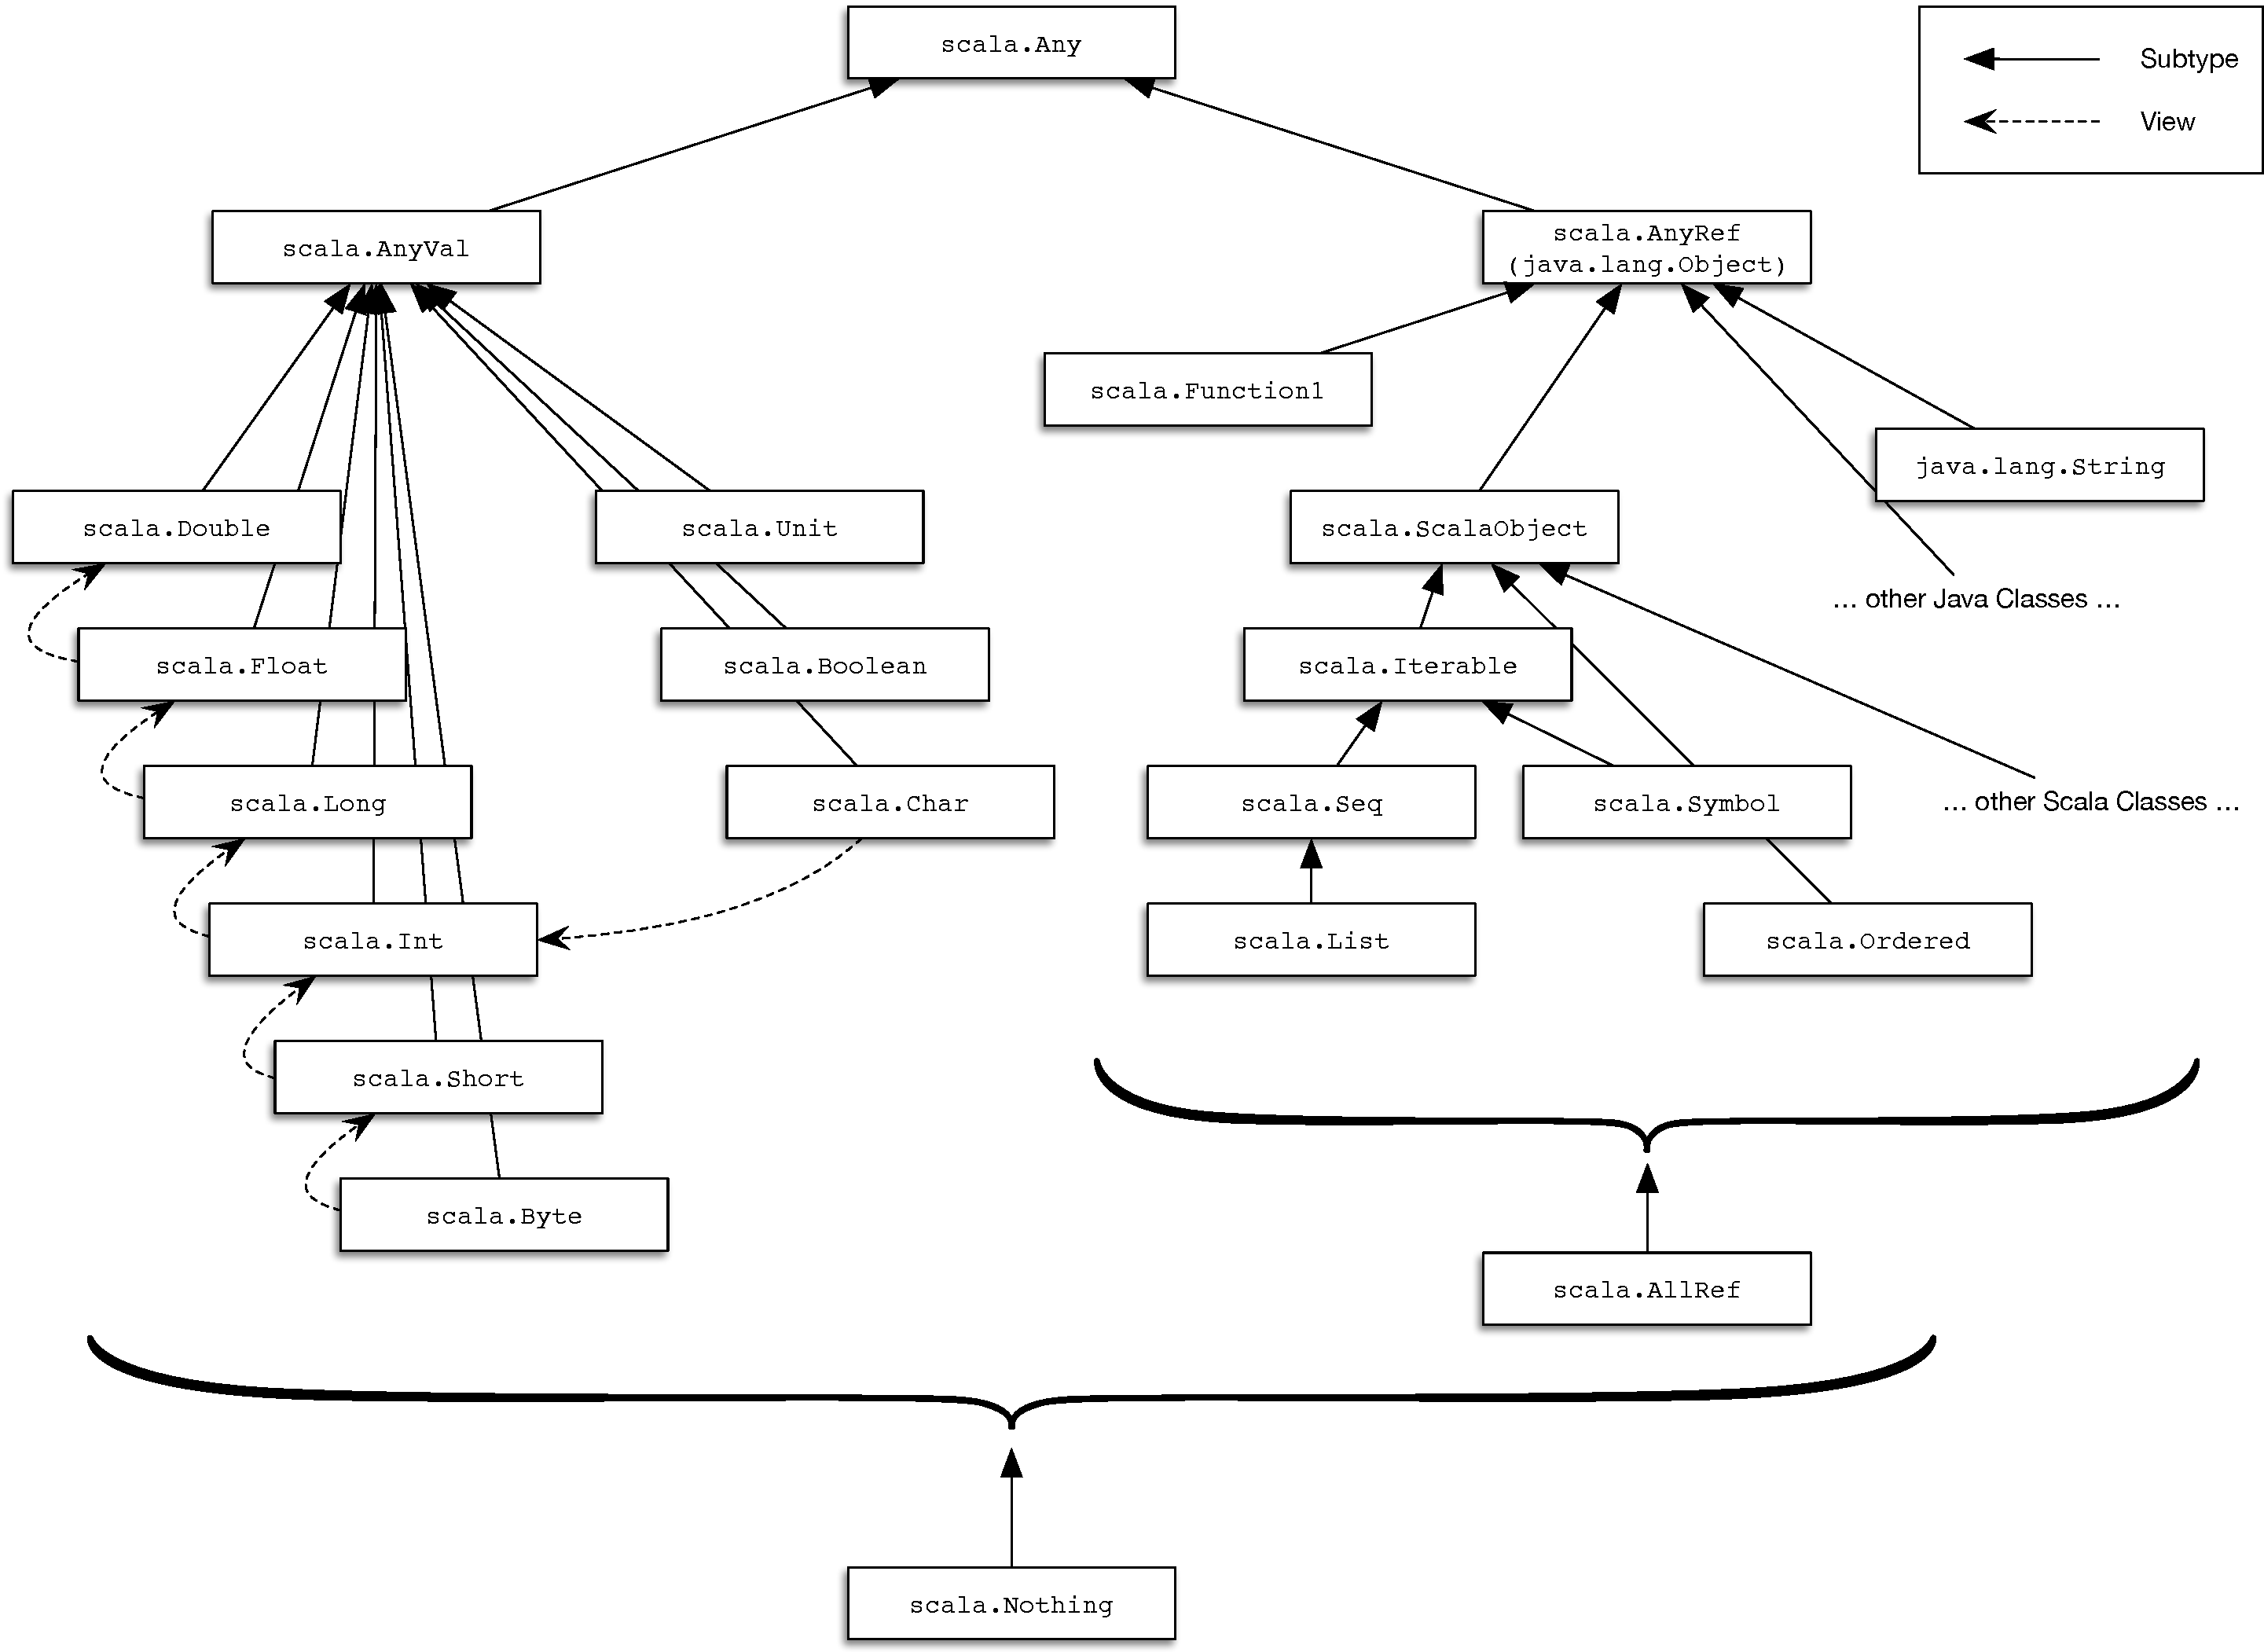
\includegraphics[width=\textwidth]{scala_classes}
    \caption{A visual representation of Scala's class hierarchy}
    \label{fig:example}
  \end{figure} 

\subsection{Pattern Matching in an Object-Oriented Setting}
Unlike Java and other object-oriented programming languages, Scala implements pattern matching. That is, Scala provides the programmer with a natural and functional-like mechanism for ``creating structured data representations similar to algebraic data types and a decomposition mechanism based on pattern matching.'' \\\\
Since Scala is an object-oriented programming language, it does not have algebraic data types. Instead, Scala creates structured data representations through the \texttt{\textbf{case}} modifier. If $\textbf{case}$ precedes the definition of a class, a factory method with the same arguments as the primary class constructor is automatically defined. For example, in Figure 4, since the \texttt{\textbf{Num}} and \texttt{\textbf{Plus}} classes are defined with the \texttt{\textbf{case}} modifier, we can define an “anonymous” \textbf{Num} object without using the \textbf{new} keyword. As the reader can see, factory methods are very similar in structure to the constructors of algebraic data types. In fact, factory methods serve the same purpose as constructors when pattern matching.\\\\
Scala's pattern matching expressions can decompose the factory method constructors as patterns. The syntax for pattern matching expressions is 
\[
    \texttt{x \textbf{case} \{ \textbf{case} $p_1 => e_1$ \textbf{case} $p_1 => e_1$ ... \}}
\]
This syntax matches the object \texttt{x} against the patterns $p_1, p_2, ...$ in order. Each $p_1$ is of the form $FactoryMethod(x_1, x_2, …, x_n)$, where $FactoryMethod$ refers to the factory method constructors discussed previously. When a match $p_i$ is found, then $e_i$ is executed. For example, in Figure 5, the \texttt{eval} function matches \texttt{term} against \texttt{Num(x)} and \texttt{Plus(left, right)} (the constructors are from Figure 4).

  \begin{figure}[h]
    \centering
    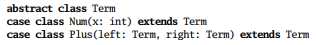
\includegraphics[width=\columnwidth]{abstract_class}
    \caption{example}
    \label{fig:example}
  \end{figure}

  \begin{figure}[h]
    \centering
    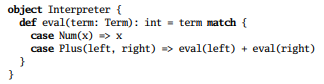
\includegraphics[width=\columnwidth]{pattern_match}
    \caption{}
    \label{fig:example}
  \end{figure}
Note: unlike Java, writing a simple language interpreter in Scala is almost as easy as writing an interpreter in SML. Examples of pattern matching being used for an interpreter can be seen in the calculator program we wrote.

\subsection{Views}
Views are used to implictly convert one type to another. A view is implemented with a method that takes in an arguemnt of one type and returns an object of another type. The only difference between a view method and a normal method is that view methods require the \texttt{implicit} modifier, which goes before the method definition. This modifier allows the Scala compiler to know that it is the implcit conversion method when converting from one type to another. Scala implictly applies a view to an expression, $e$ of type $T$, when one of the following cases occur:
\begin{itemize}
    \item The expected type of $e$ is not of type $T$.
    \item A member selected from $e$ is not a member of $T$.
\end{itemize}  
For example, in Figure 7, \texttt{listToSet} is the view that converts \texttt{GenList[T]} to \texttt{Set[T]}. The compiler inserts applications of the view onto \texttt{xs}.
\begin{figure}
  
  \inputminted{Scala}{examples/Set.scala}
  \caption{An example of views and implcit conversions.}
  \label{lst:nats-example}
\end{figure}
% TODO
% singleton objects - DONE

% unified object model -DONE

% pattern matching in an object oriented setting -DONE

% Abstraction: -NOT DONE
% - subtypes and polymorphism
% - Traits and classes.
%   - A trait do encapsulate state. They just define methods or variables that you
%     have to have but don't provide instantiated values for those.
%   -Classes require implementations or values for everything.

% Multiple inheritance with mixins. (Small paragraph right after abstractions) -NOT DONE

% Views in Scala implement something close to SML's signatures or Haskell's
% typeclasses. -DONE

% 4. report on peano arithmetic calculator.
\section{Engagement: Peano Arithmetic Calculator}
\label{sec:engag-peano-arithm}

% 5. should encapsulate discussion of current status
\section{Discussion}
\label{sec:discussion}

\subsection{Current Status of Work}
After 15 years, Scala has been regularly updated and is currently at stable
release version 2.12.8. Over this period, the core principles of Scala have
remained the same. Scala has achieved widespread adoption in the industry with
companies such as Twitter and Apple utilizing the language. Moreover, Scala has
both a large academic and non-academic user base. The language is often cited or
used in computer science research. In addition, Scala's user community is
thriving. there exist chatrooms, subreddits, and research conferences devoted
entirely to Scala. Numerous libraries, tutorials, and guides are run and
maintained by the community. The main community page can be found at:
https://www.scala-lang.org/community/. A detailed, updated, and easy to read
documentation can be found at: https://docs.scala-lang.org/. Finally, there are
dedicated installers/installation guides for all operating systems at:
https://www.scala-lang.org/download/.


\bibliographystyle{IEEEtran}
\bibliography{scala_project}

\end{document}

%%% Local Variables:
%%% mode: latex
%%% TeX-master: t
%%% TeX-command-extra-options: "-shell-escape"
%%% End:
